% Шаблон (версия от 15.02.2016) предназначен 
% для использования студентами каф. ПМиИ СамГТУ 
% при оформлении отчетов по лабораторным работам. 
% Для настройки пакета listigs использовался материал 
% статьи Михаила Конника aka virens
% <http://mydebianblog.blogspot.ru/2012/12/latex.html>
% Copyright (c) 2016 by Mikhail Saushkin (msaushkin@gmail.com) 
% All rights reserved except the rights granted by the
% Creative Commons Attribution 4.0 International Licence
% <https://creativecommons.org/licenses/by/4.0/>
% Свежая версия шаблона здесь <https://www.overleaf.com/read/sqvxbnhgxxdm>
\documentclass[14pt,a4paper,report]{ncc}
\usepackage[a4paper, mag=1000, left=2.5cm, right=1cm, top=2cm, bottom=2cm, headsep=0.7cm, footskip=1cm]{geometry}
\usepackage[utf8]{inputenc}
\usepackage[english,russian]{babel}
\usepackage{indentfirst}
\usepackage[dvipsnames]{xcolor}
\usepackage[colorlinks]{hyperref}
\usepackage{listings} 
\usepackage{caption}
\usepackage{amssymb}
\usepackage{tcolorbox}
\DeclareCaptionFont{white}{\color{white}} %% это сделает текст заголовка белым
%% код ниже нарисует серую рамочку вокруг заголовка кода.
\usepackage{color} %% это для отображения цвета в коде
\DeclareCaptionFormat{listing}{\colorbox{gray}{\parbox{\textwidth}{#1#2#3}}}
\captionsetup[lstlisting]{format=listing,labelfont=white,textfont=white}
\lstset{% Собственно настройки вида листинга
inputencoding=utf8, extendedchars=\true, keepspaces = true, % поддержка кириллицы и пробелов в комментариях
language=C++,            % выбор языка для подсветки (здесь это Pascal)
numberstyle =\tiny
basicstyle=\small\sffamily, % размер и начертание шрифта для подсветки кода
keywordstyle =\color{ForestGreen},
numbers=left,               % где поставить нумерацию строк (слева\справа)
numberstyle=\tiny,          % размер шрифта для номеров строк
stepnumber=1,               % размер шага между двумя номерами строк
numbersep=5pt,              % как далеко отстоят номера строк от подсвечиваемого кода
backgroundcolor=\color{white}, % цвет фона подсветки - используем \usepackage{color}
showspaces=false,           % показывать или нет пробелы специальными отступами
showstringspaces=false,     % показывать или нет пробелы в строках
showtabs=false,             % показывать или нет табуляцию в строках
frame=single,               % рисовать рамку вокруг кода
tabsize=2,                  % размер табуляции по умолчанию равен 2 пробелам
captionpos=t,               % позиция заголовка вверху [t] или внизу [b] 
breaklines=true,            % автоматически переносить строки (да\нет)
breakatwhitespace=false,    % переносить строки только если есть пробел
escapeinside={\%*}{*)}      % если нужно добавить комментарии в коде
}

\begin{document}
% Переоформление некоторых стандартных названий
%\renewcommand{\chaptername}{Лабораторная работа}
\def\contentsname{Содержание}

% Оформление титульного листа
\begin{titlepage}
\begin{center}
\textsc{ФГОУ ВО Уральский Федеральный Университет \\ имени первого Президента России Б.Н.Ельцина\\[5mm]
Физико-технологический институт\\[2mm]
Кафедра теоретической физики и прикладной математики}

\vfill

\textbf{ОТЧЁТ ПО ЛАБОРАТОРНОЙ РАБОТЕ №4\\[3mm]
«НАЗВАНИЕ»\\[6mm]
}
\end{center}

\hfill
\begin{minipage}{.5\textwidth}
Студент:\\[2mm] 
Вялова С.А.\\
группа: ФтМ-170403 \\[5mm]

Преподаватель:\\[2mm] 
д.ф.-м.н., профессор\\
Мазуренко Владимир Владимирович\\[5mm]

Консультант:\\[2mm] 
н.с.\\
Сотников Олег Михайлович\\

\end{minipage}%
\vfill
\begin{center}
\today  \\
%\theyear\, г.
 Екатеринбург.
\end{center}
\end{titlepage}

% Содержание
\tableofcontents
\newpage
\chapter{Моделирование атомной структуры реальных кристаллов}
\section{Цель работы}


Разработка программы для моделирования основного состояния двумерных решеток, в которых частицы взаимодействуют через потенциал Леннарда-Джонса. Рассмотрение квадратной и треугольной решетки с одинаковой плотностью атомов.
\

В ходе выполнения работы необходимо реализовать следующие пункты:
\begin{itemize}
\item Определить энергии треугольной и квадратной решеток при различных линейных размеров решеток;
\item вычислить плотность системы в каждом случае;
\item выяснить, какова зависимость плотности решетки от линейных размеров решетки;
\item выяснить, энергия какой из рассматриваемых решеток меньше.
\end{itemize}

\

\newpage\section{Теоретическая часть }
\subsection{Потенциал Леннарда-Джонса}
%text
Потенциал Леннарда-Джонса представляет собой простую модель парного взаимодействия неполярных молекул, описывающая зависимость энергии взаимодействия двух частиц от расстояния между ними.
Потенциал был предложен Леннардом-Джонсом первоначально для исследования термодинамических свойств инертных газов. Наиболее часто используется так называемый (6-12)-потенциал Леннарда-Джонса, записанный в форме 
\
\begin{equation}
 U = 4 \cdot \varepsilon \cdot [(\sigma/r)^{12} - (\sigma/r)^{6}  ] ,
 \end{equation} 
где $\varepsilon$ - глубина потенциальной ямы, $\sigma$ - значение расстояния между частицами, при котором потенциал равен нулю. Шестая степень убывания отвечает электростатическому диполь-дипольному и дисперсионному притяжению; двенадцатая степень убывания потенциала моделирует достаточно жесткое отталкивание и выбрана из соображений математического удобства.
\


%\caption{Зависимость температуры системы от шага по времени.}

\newpage
\subsection{Описание  методов}
%text
В ходе работы необходимо исследовать треугольную решетку с дефектами типа вакансий. Для этого был видоизменен программный код для программы моделирования динамики двумерной системы частиц, взаимодействующих через потенциал Леннарда-Джонса, а также программы моделирования такой же системы частиц, но при использовании алгоритма Метрополиса.
\

Вакансия в заданной решетке задаётся путем исключения одной или нескольких частиц из рассмотрения. Число вакансий, а также расположение их выбирается программой произвольным образом: генерируется случайное число $n_deleted$ от $[1, \frac{n}{4}]$ ($n$ - число частиц в системе), задающее количество вакансий, а также массив i_deleted размерностью n_deleted, элементы которого также представляют из себя набор произвольных чисел, выбранных в промежутке от $[1, n]$. Число частиц в системе, соответственно, уменьшается на число вакансий, а массив координат частиц смещается, из него исключаются все элементы, соответствующие вакансиям.
\

После чего запускается либо динамика частиц при использовании алгорима Верле, либо квазидинамика, реализованная при использовании алгоритма Метрополиса.

Пусть $L_x$ - ширина треугольной решетки, $n_c$ - число частиц в каждой строке или столбце. Столбцы треугольной решетки отстоят друг от друга на $a={L_x}/{n_c}$, а каждую строку разделяет расстояние $\frac{\sqrt{3}}{2} a$. В каждой строке узлы смещены на $\frac{a}{2}$ относительно предыдущей строки. Высота треугольной решетки составляет $L_y=\frac{\sqrt{3}L_x}{2}$, а общее число частиц в системе составляет $N={n_c}^2$. 
\
Параметры для квадратной решетки подбираются исходя из требования равенства плотностей  треугольной и квадратной решеток. Таким образом, сторона квадратной решетки $L=\sqrt{L_x \cdot L_y}$.
\

Энергия решетки вычисляется через потенциал Леннарда-Джонса следующим образом:
\begin{equation}
E=4 \varepsilon \sum\limits_{i=1}^N \sum\limits_{s=i+1}^N{ [(\sigma/\vec{r}_{is})^{12} - (\sigma/\vec{r}_{is})^{6}  ]}
\end{equation}
\subsection{Результаты моделирования квазидинамики через алгоритм Метрополиса}
Система задана со следующими параметрами:
\begin{itemize}
\item Линейные размеры системы по горизонтали $L_x=7$, линейные размеры системы по вертикали $L_y=\frac{\sqrt{3}}{2}L_x$;
\item число частиц $n=81$;
\item $\sigma=0.699$;
\item температурный множитель$kT=0,00005$;
\item число шагов алгоритма Метрополиса $N=10000$;
\end{itemize}

Система в начальный момент времени представлена на рисунке\ref{ris:image1}. Решетка, как можно увидеть, содержит 6 вакансий. Через некоторое количество шагов система пришла к виду, изображенному на рисунке \ref{ris:image2}, из которого видно, как вакансия влияет на эволюцию системы в ходе моделирования: решетка вновь стремится занять наиболее выгодное положение - принять треугольную конфигурацию. 
\begin{figure}[h]
\center{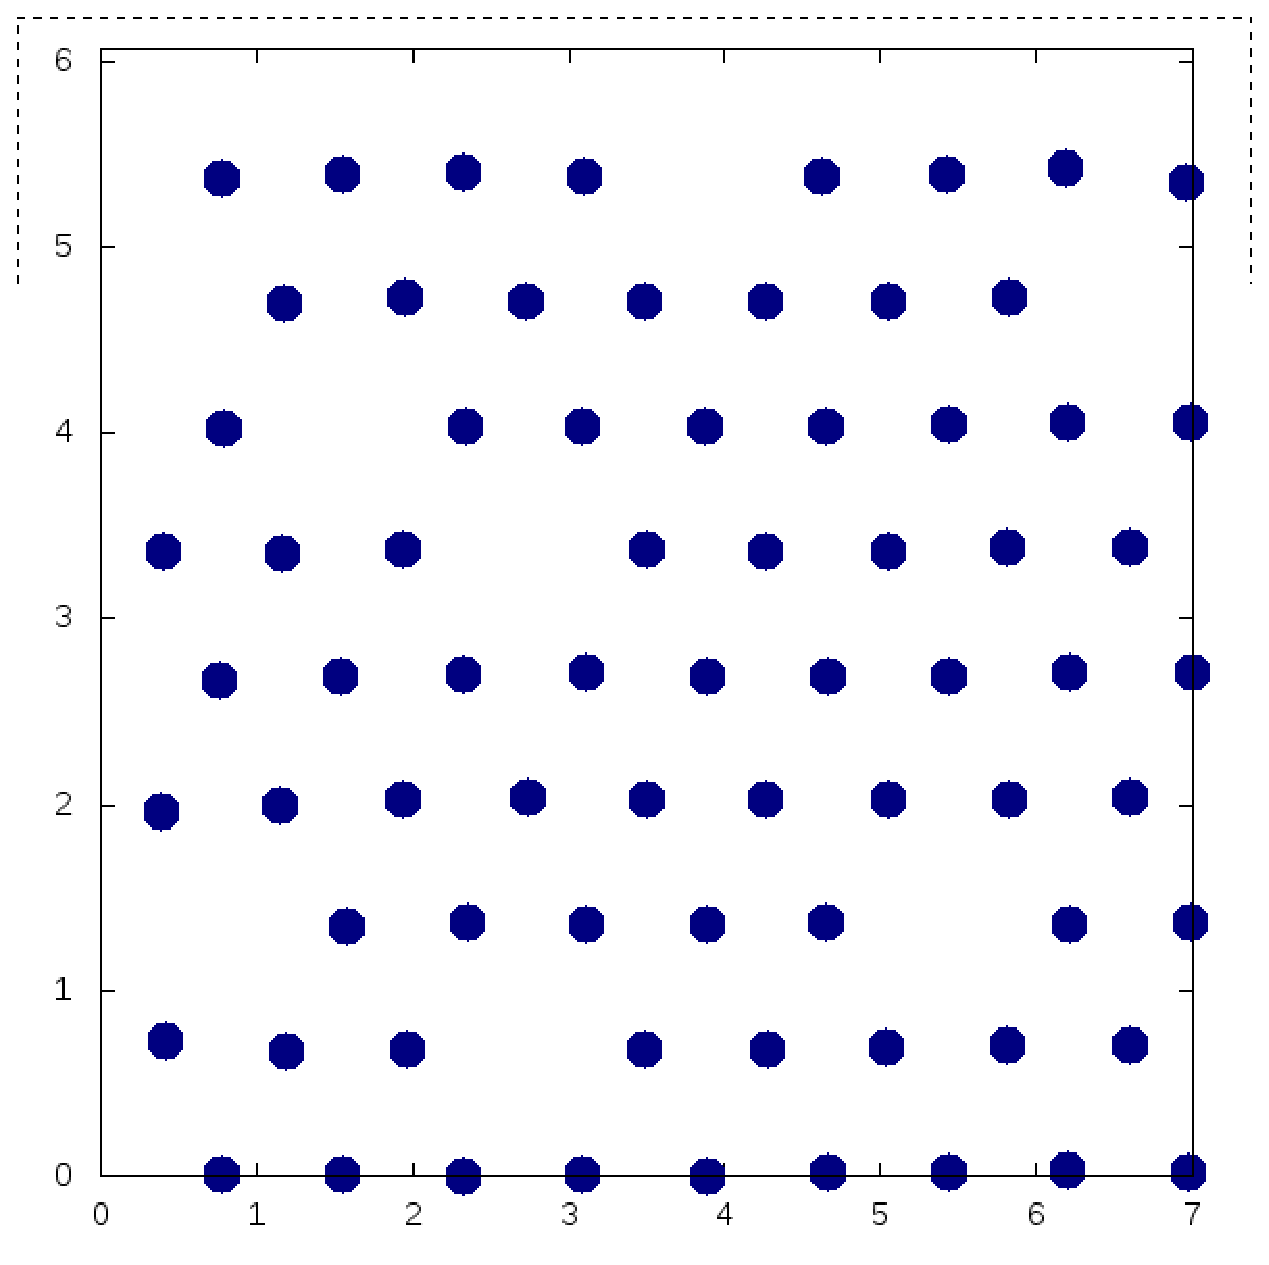
\includegraphics[width=1\linewidth]{/pictures/system_8_vac_kT00005}}
\caption{Система с 6-ю вакансиями в начальный момент времени.}
\label{ris:image1}
\end{figure}
\begin{figure}[h]
\center{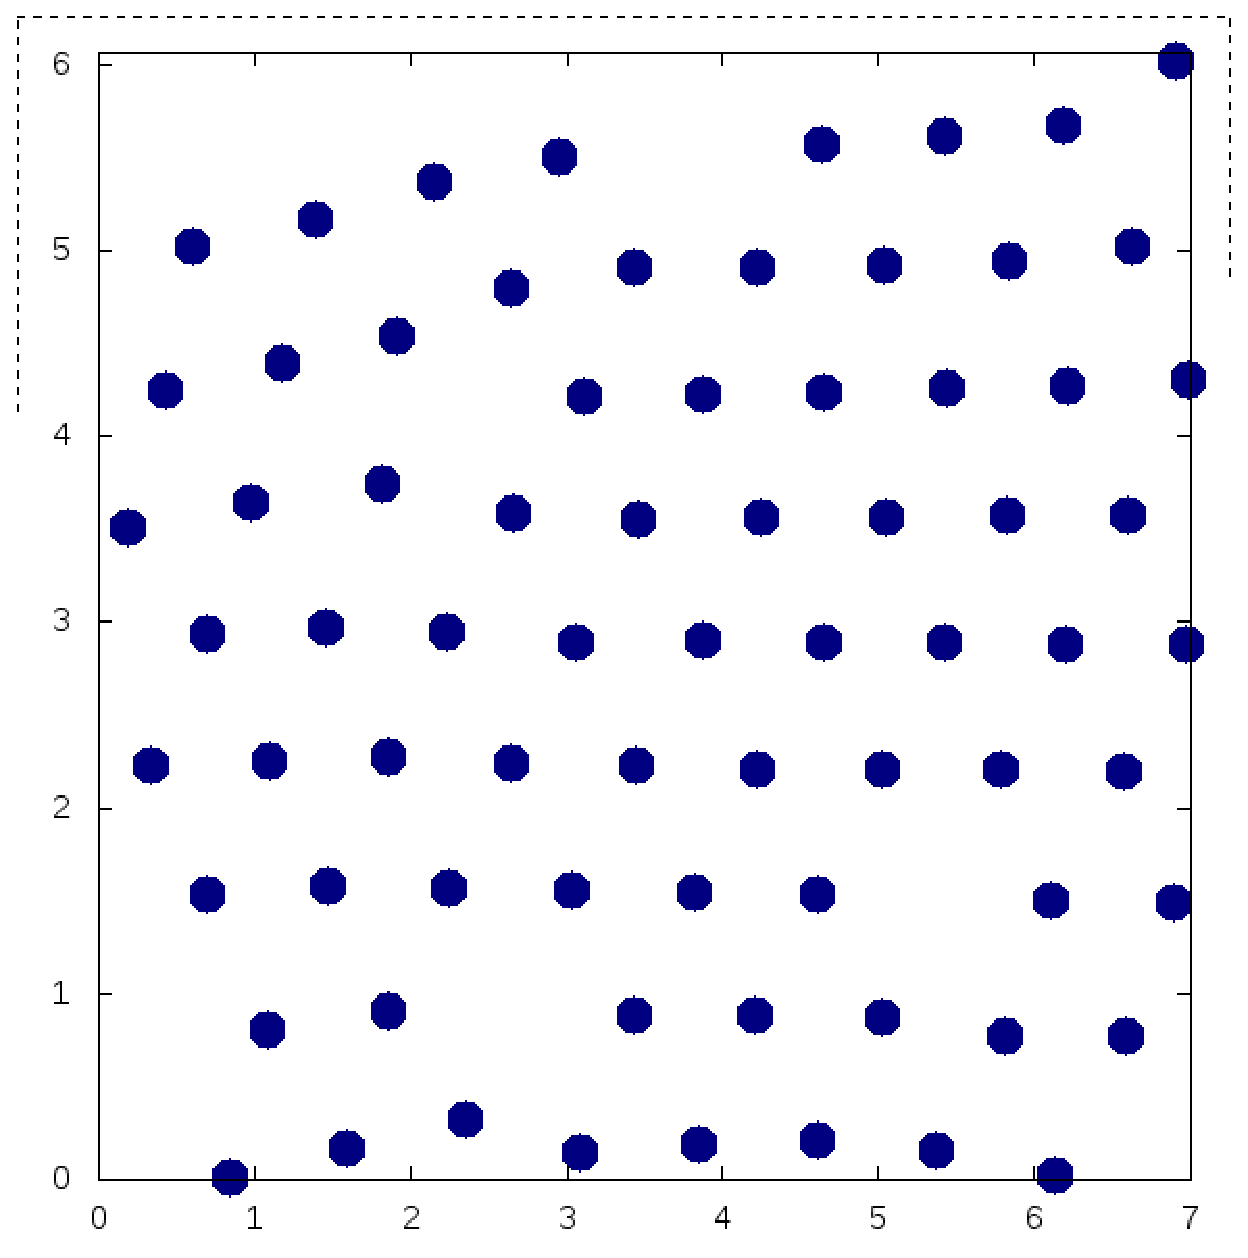
\includegraphics[width=1\linewidth]{pictures/system_dynamic_8_vac_kT00005}}
\caption{Система с 6-ю вакансиями в ходе моделирования.}
\label{ris:image2}
\end{figure}
\

Рассмотрим теперь график зависимости энергии системы от шага моделирования (\ref{ris:image3}). Система, как можно судить по данной зависимости, стремится прийти к энергетически наиболее выгодной конфигурации. 
\begin{figure}[h]
\center{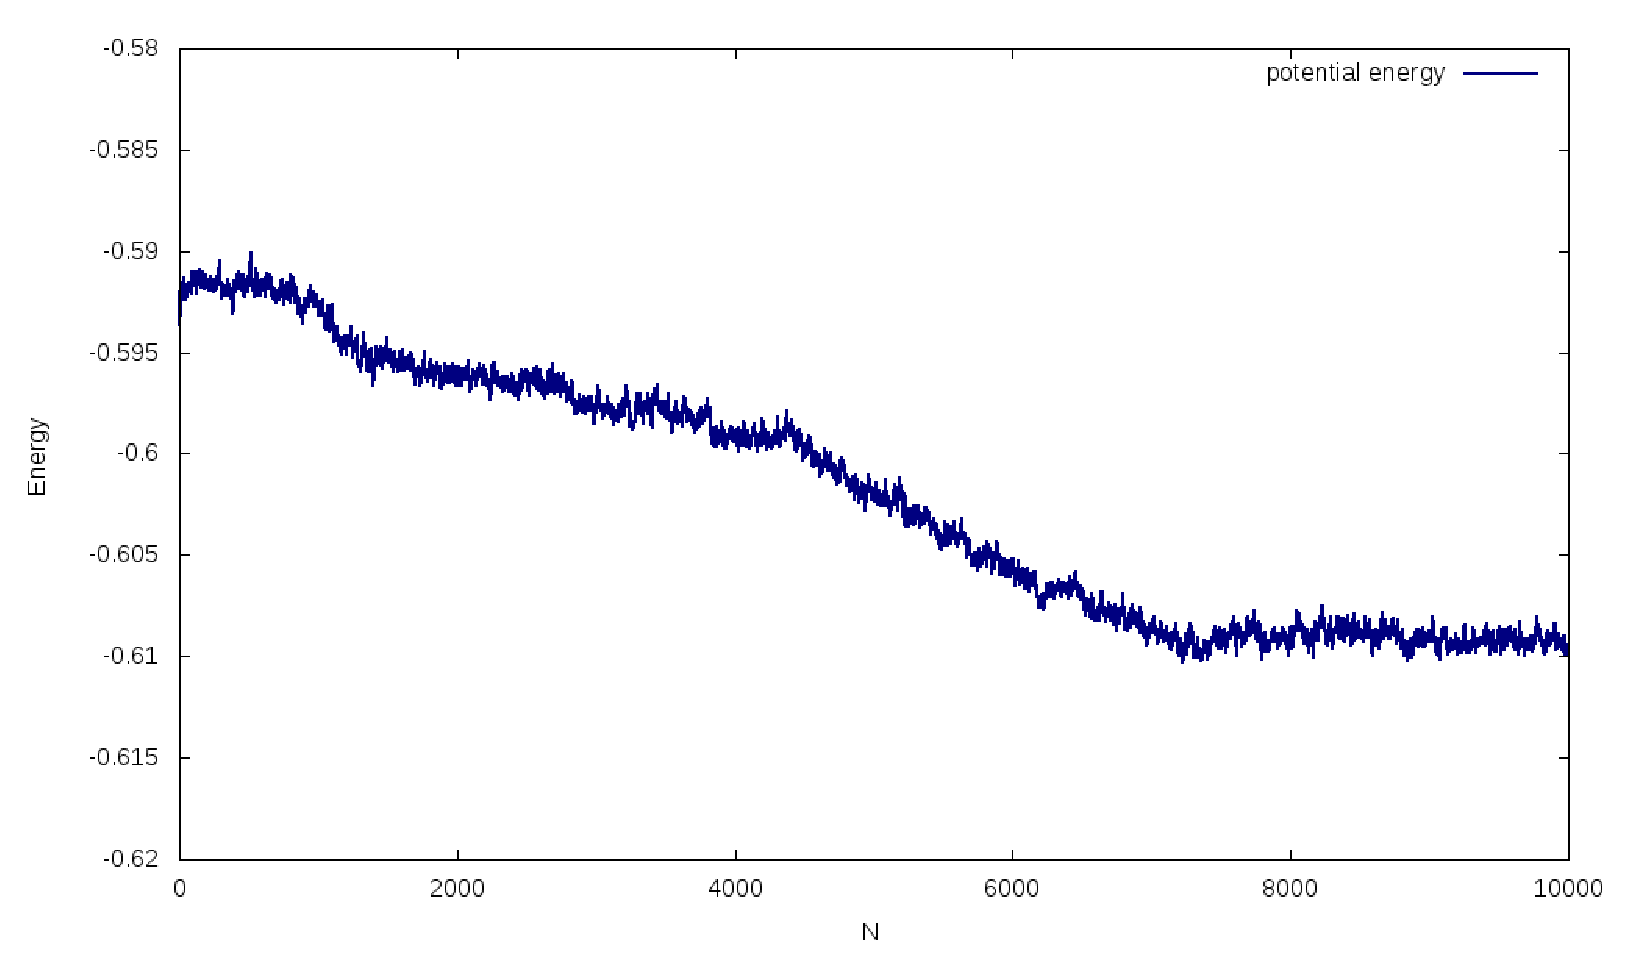
\includegraphics[width=1\linewidth]{pictures/energy_8_vac_kT00005}}
\caption{График зависимости энергии системы с 6-ю вакансиями от шага моделирования.}
\label{ris:image3}
\end{figure}
\
Более того, сразу можно сказать, что энергия системы с вакансиями выше, нежели энергия такой же системы без вакансий: расчёт основного состояния системы был проведен при помощи программы, разработанной для проведения лабораторной работы №2 (рисунок \ref{ris:image3}).
\begin{figure}[h]
\center{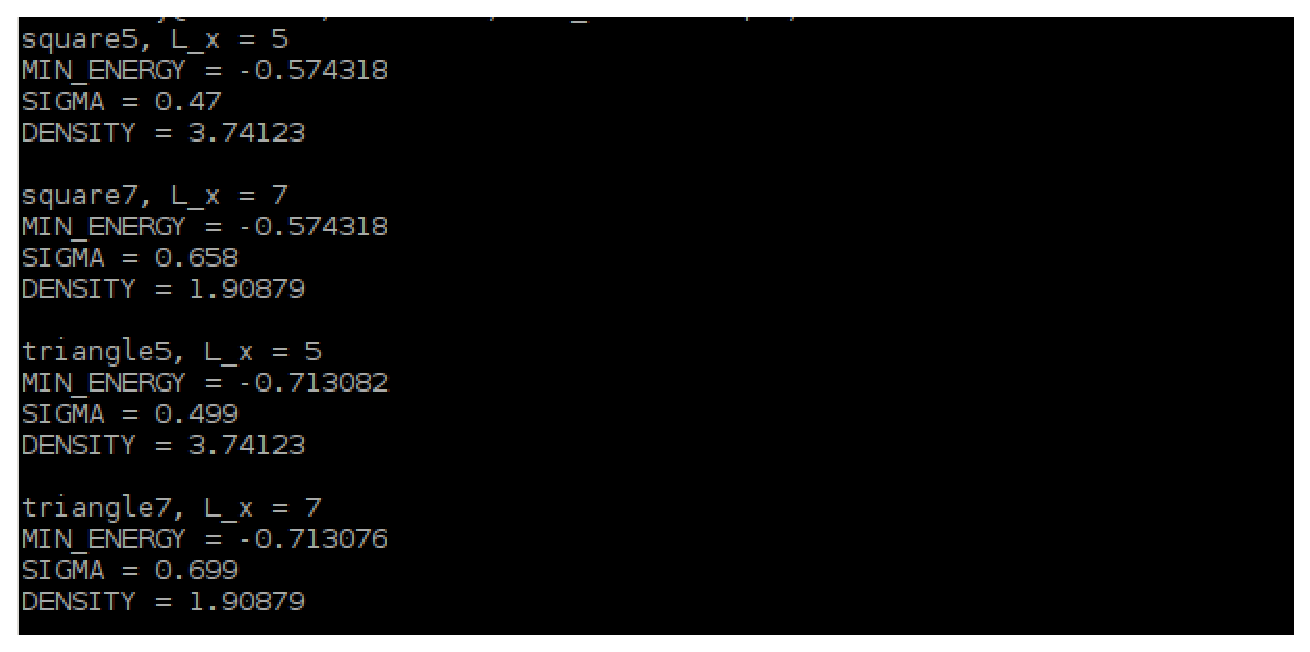
\includegraphics[width=1\linewidth]{pictures/program_lab2}}
\caption{Результат расчёта основного состояния треугольной решетки.}
\label{ris:image4}
\end{figure}
Из графика зависимости энергии системы также можно сделать вывод, что энергия равновесного, к которой пришла данная система с вакансиями, выше энергии основного состояния такой же системы без вакансий.
\

График среднеквадратического отклонения частиц в ходе моделирования представлен на рисунке \ref{ris:image5}. Изменение координаты на каждом шагу мало, как можно увидеть, но это не мешает системе прийти к равновесному положению.
\begin{figure}[h]
\center{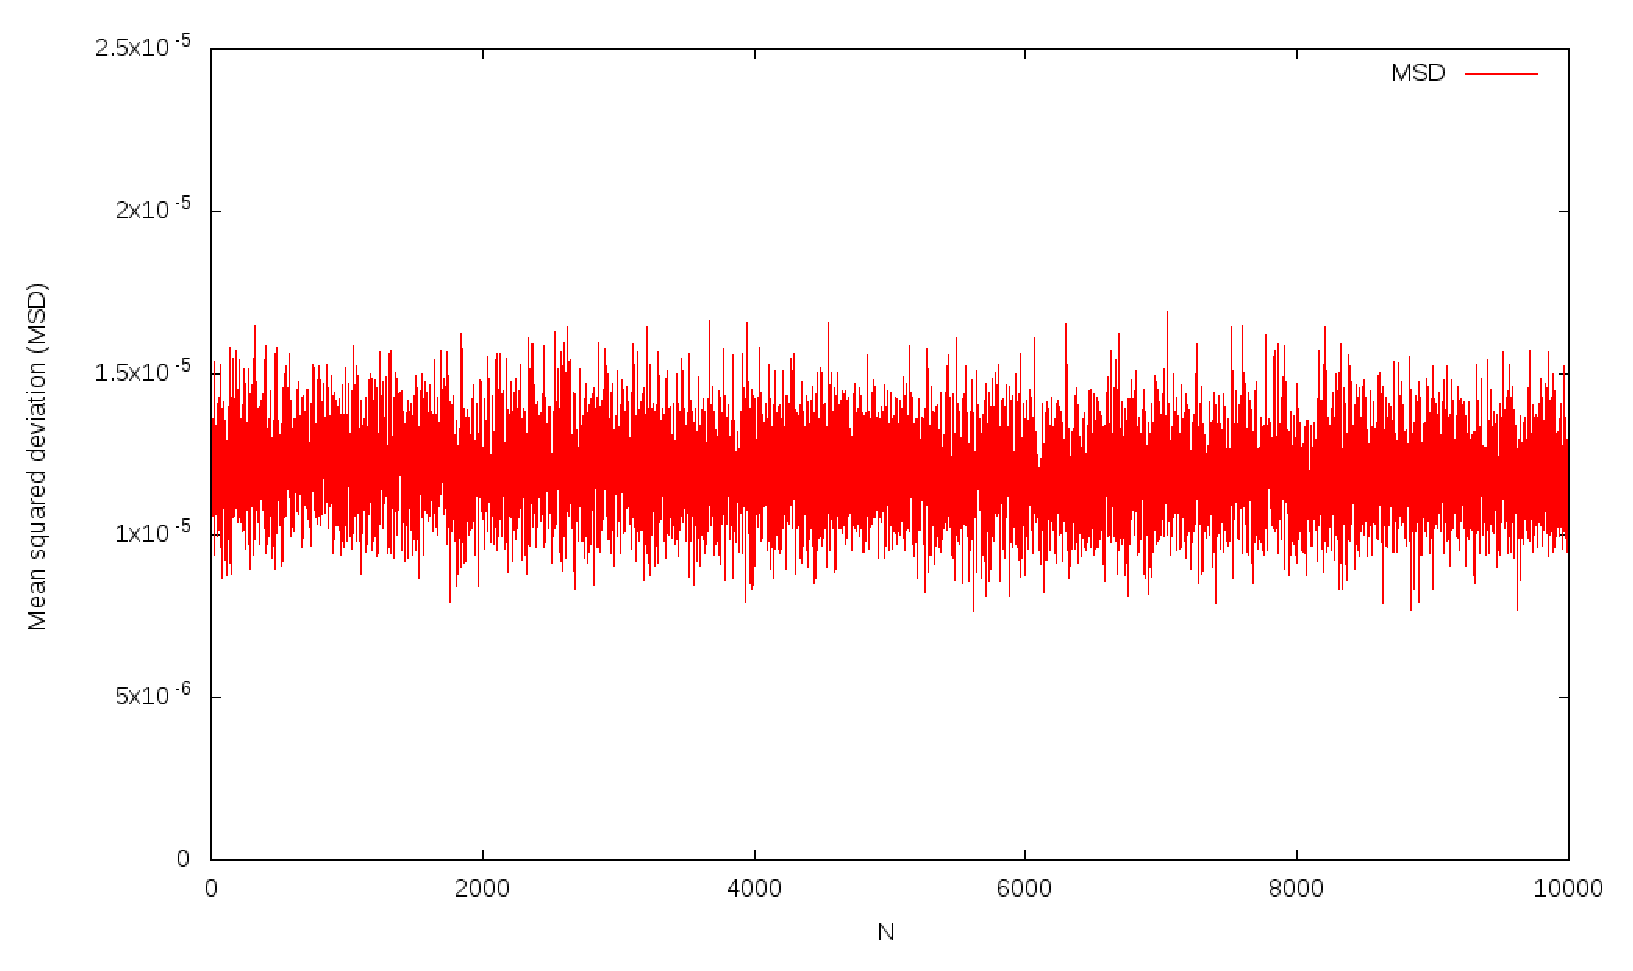
\includegraphics[width=1\linewidth]{pictures/MSD_8_vac_kT00005}}
\caption{График зависимости среднеквадратического отклонения от шага моделирования.}
\label{ris:image5}
\end{figure}
\ 

Попробуем "разрушить" решетку, увеличив температурный множитель системы kT. Система в начальный момент времени изображена на рисунке \ref{ris:image6}, в ходе моделирования - на рисунке \ref{ris:image7}. Из графика зависимости энергии системы, изображенного на рисунке \ref{ris:image8}, очевидно, что система не является стабильной - энергия повышается, это подтверждается рисунком \ref{ris:image7}.
\begin{figure}[h]
\center{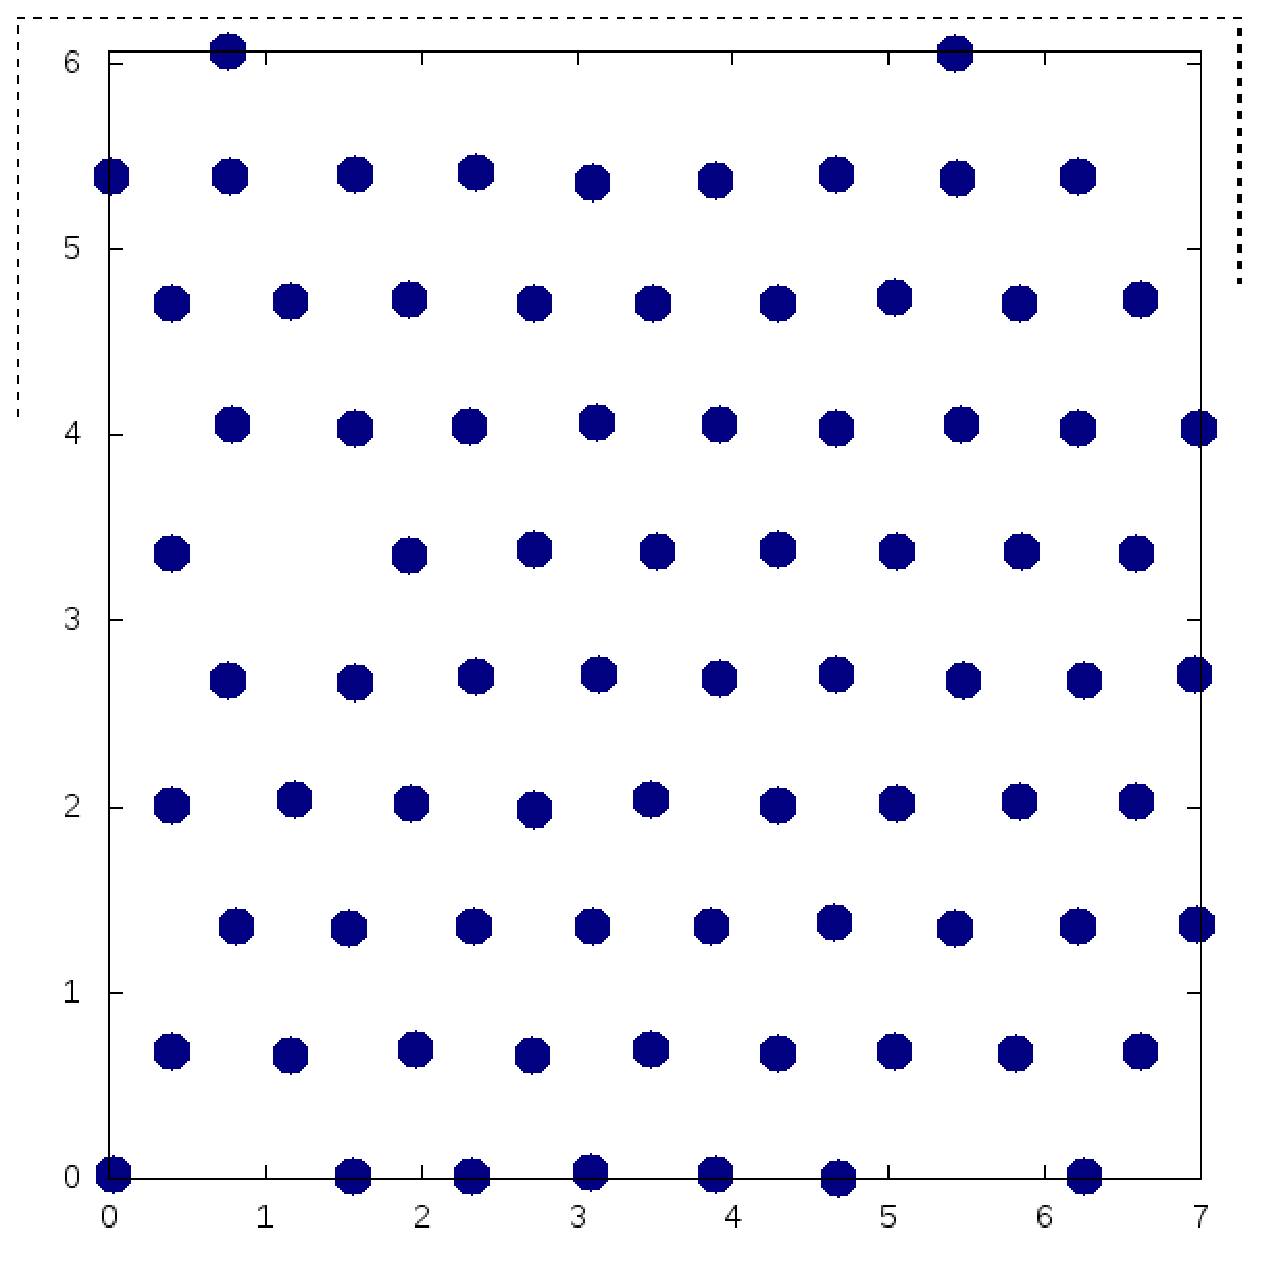
\includegraphics[width=1\linewidth]{pictures/system_8_vac_kT005}}
\caption{Система с 6-ю вакансиями в начальный момент времени.}
\label{ris:image6}
\end{figure}
\begin{figure}[h]
\center{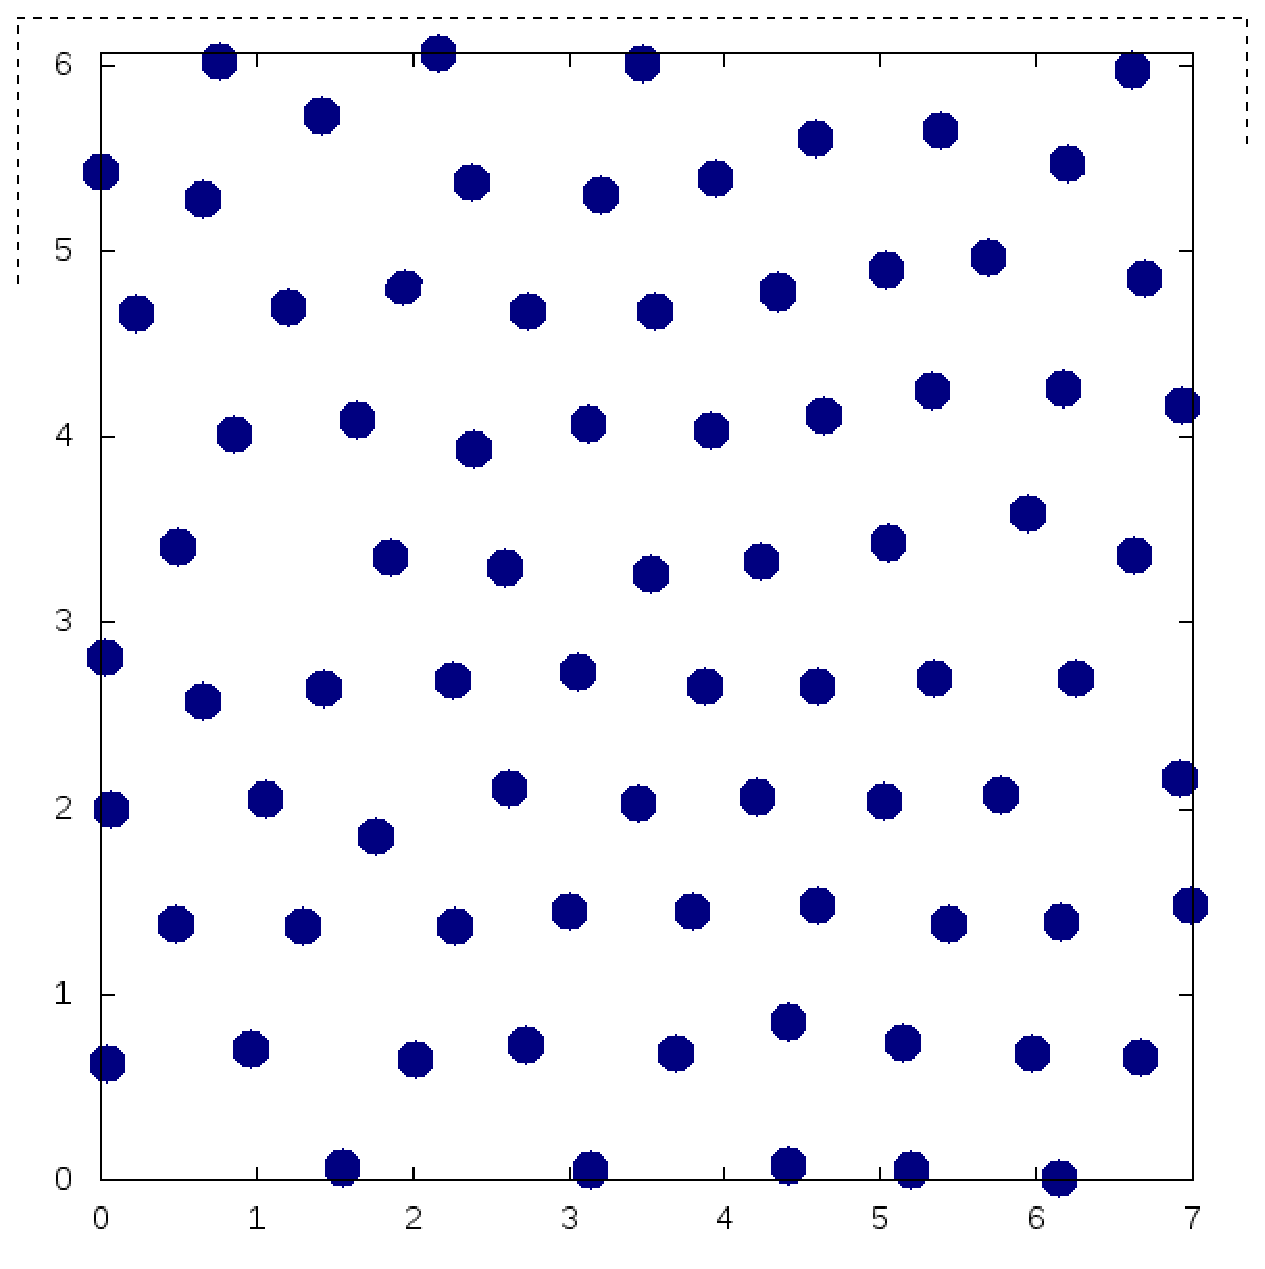
\includegraphics[width=1\linewidth]{pictures/system_dynamic_8_vac_kT005}}
\caption{Система с 6-ю вакансиями в ходе моделирования.}
\label{ris:image7}
\end{figure}
\begin{figure}[h]
\center{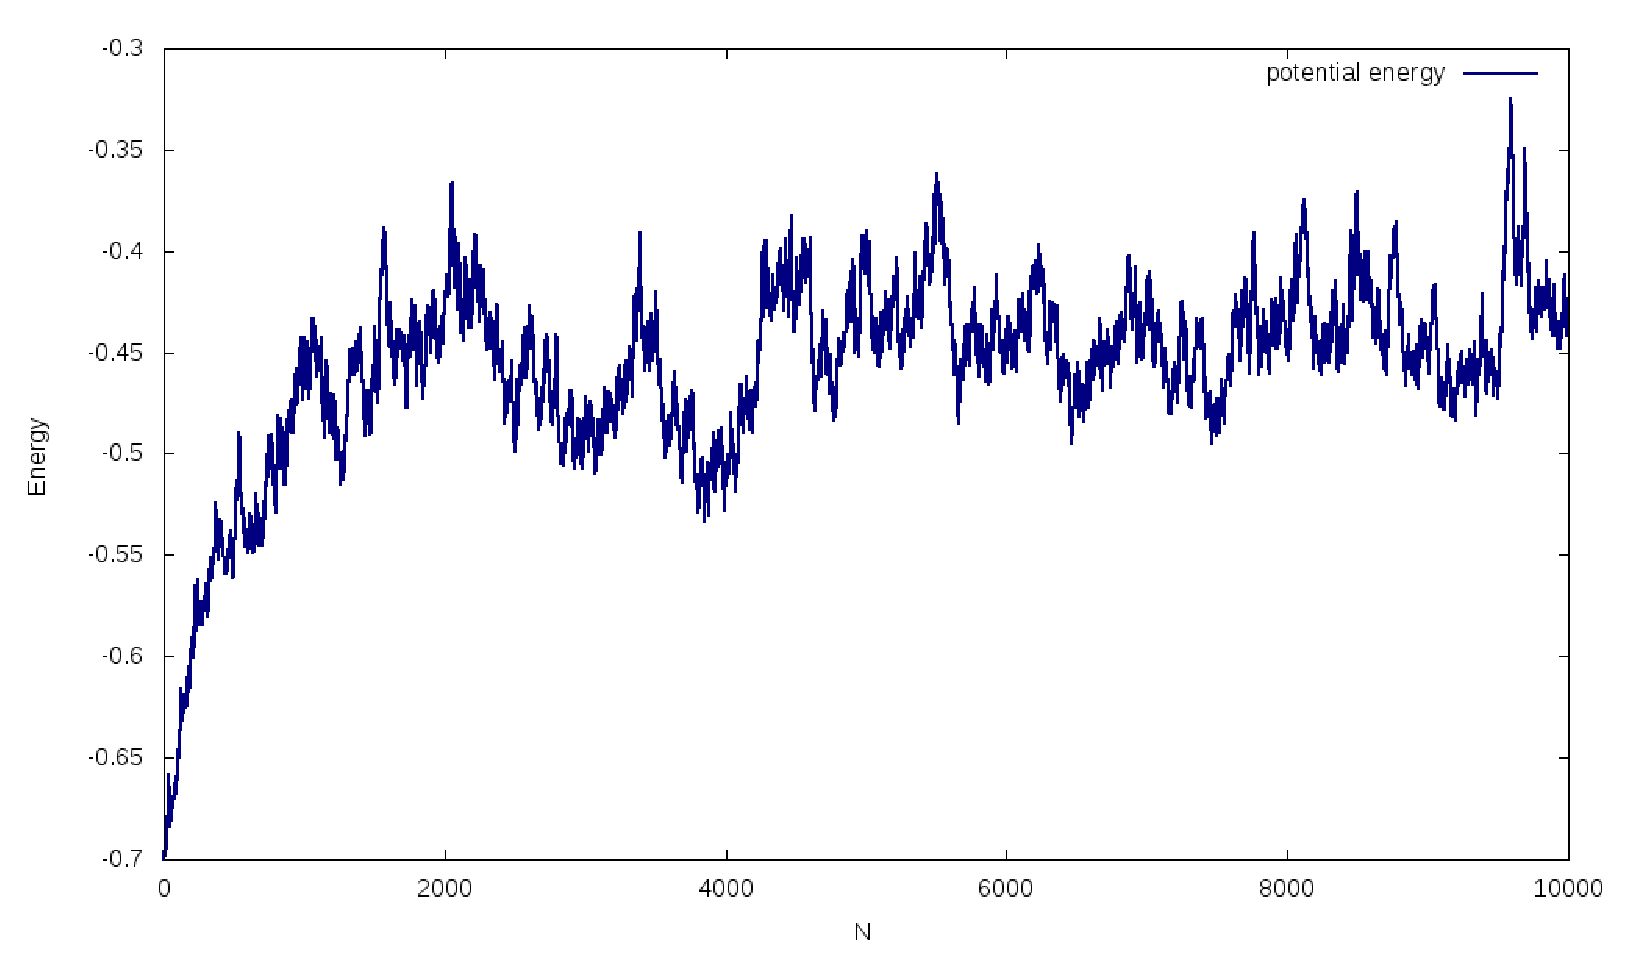
\includegraphics[width=1\linewidth]{pictures/energy_8_vac_kT005}}
\caption{График зависимости энергии системы с 6-ю вакансиями от шага моделирования.}
\label{ris:image8}
\end{figure}
Рассматривая график зависимости среднеквадратического отклонения частиц системы (рисунок \ref{ris:image9} можно сделать вывод, что частицы каждый шаг моделирования смещались на малую величину, однако это не мешало развалиться системе. 
\begin{figure}[h]
\center{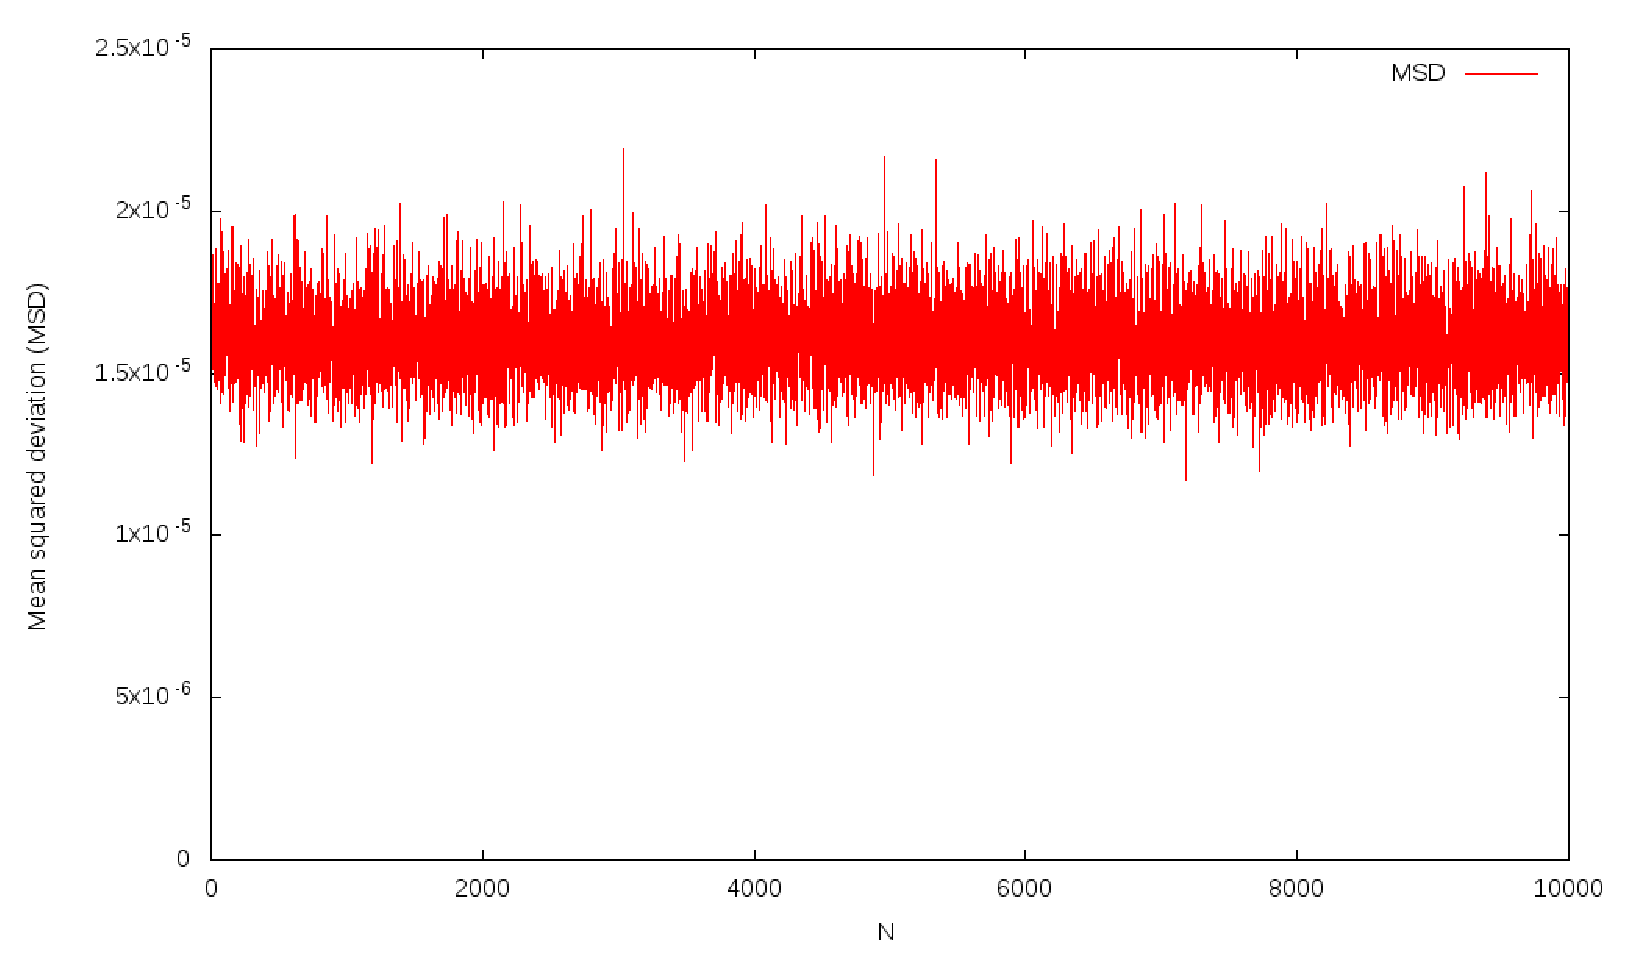
\includegraphics[width=1\linewidth]{pictures/MSD_8_vac_kT005}}
\caption{График зависимости среднеквадратического отклонения от шага моделирования.}
\label{ris:image9}
\end{figure}
\

Далее рассмотрим такую же систему, но в динамике, реализованной при использовании алгоритма Верле.
\

Начальное состояние системы представлено на рисунке \ref{ris:image10}, состояние в ходе динамики - на рисунке \ref{ris:image11}. МЯУ
\begin{figure}[h]
\center{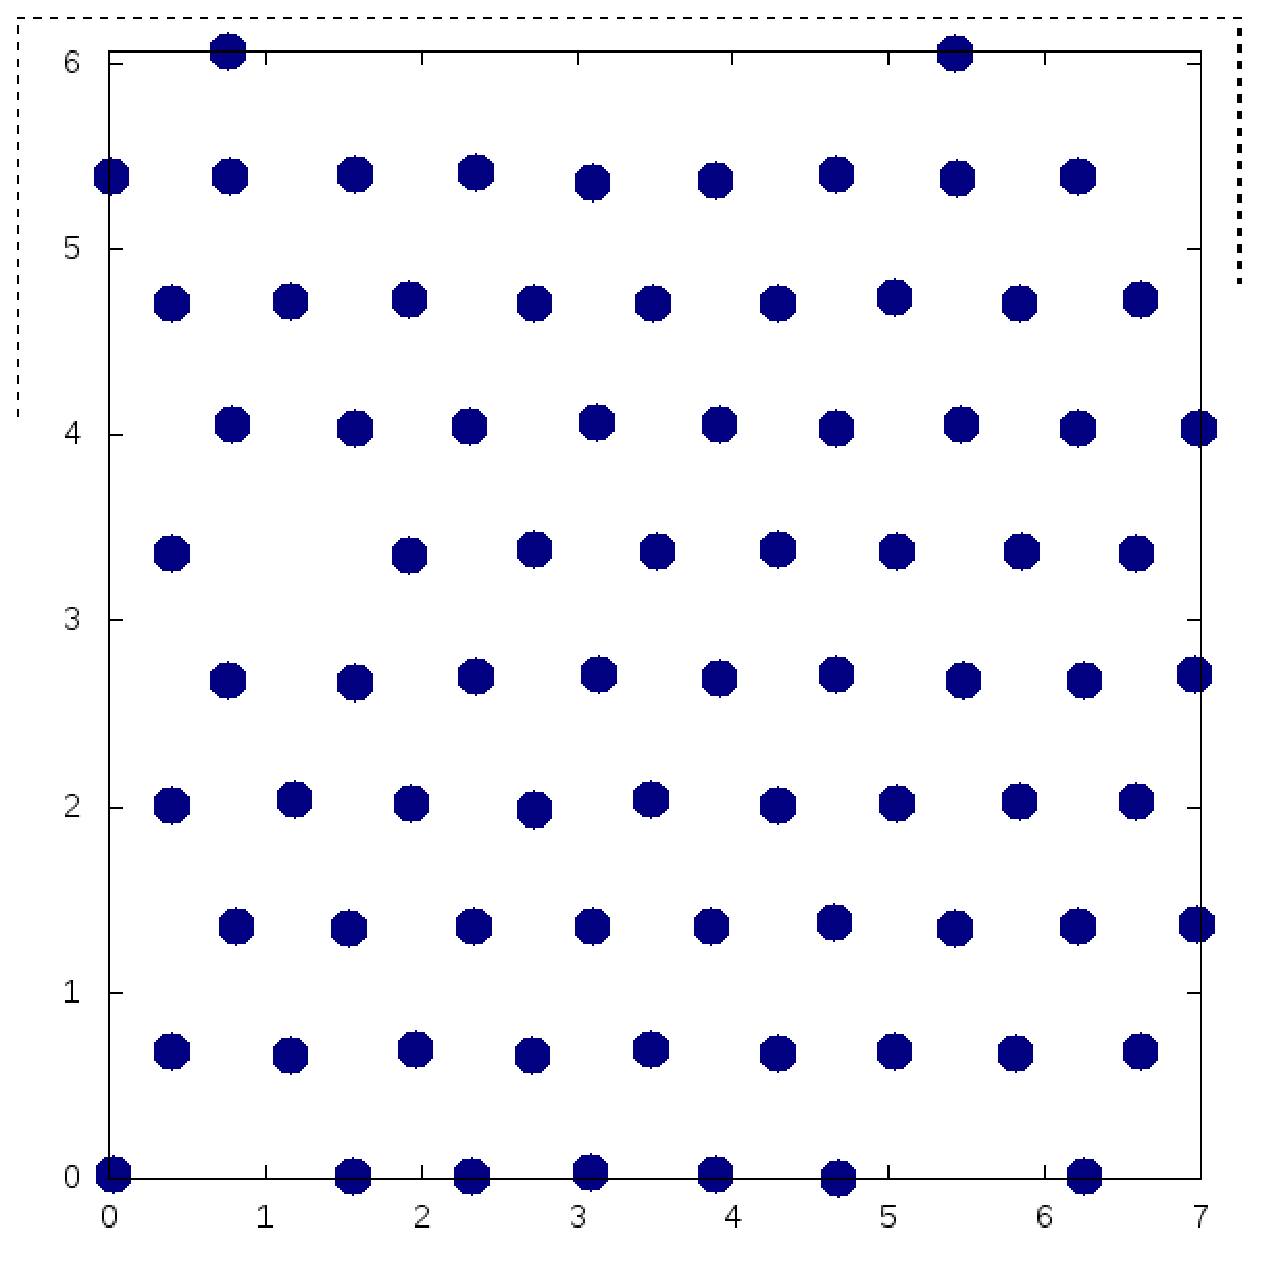
\includegraphics[width=1\linewidth]{pictures/system_8_vac_kT005}}
\caption{Система с 6-ю вакансиями в начальный момент времени.}
\label{ris:image10}
\end{figure}
\begin{figure}[h]
\center{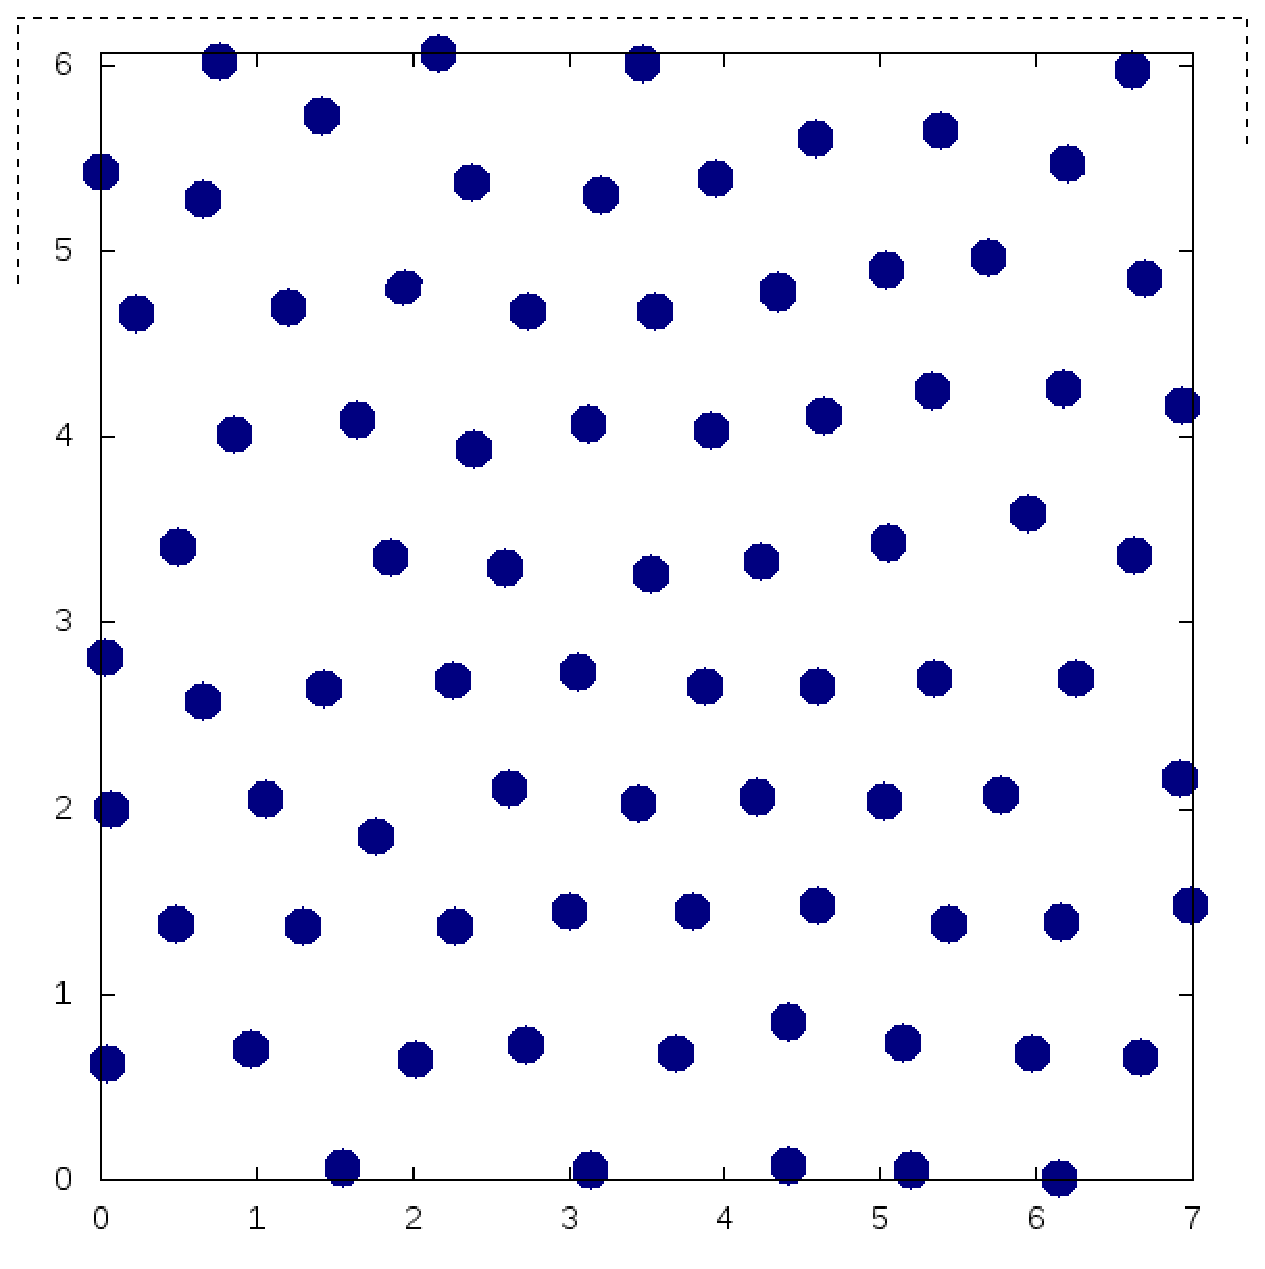
\includegraphics[width=1\linewidth]{pictures/system_dynamic_8_vac_kT005}}
\caption{Система с 6-ю вакансиями в ходе моделирования.}
\label{ris:image11}
\end{figure}
\begin{figure}[h]
\center{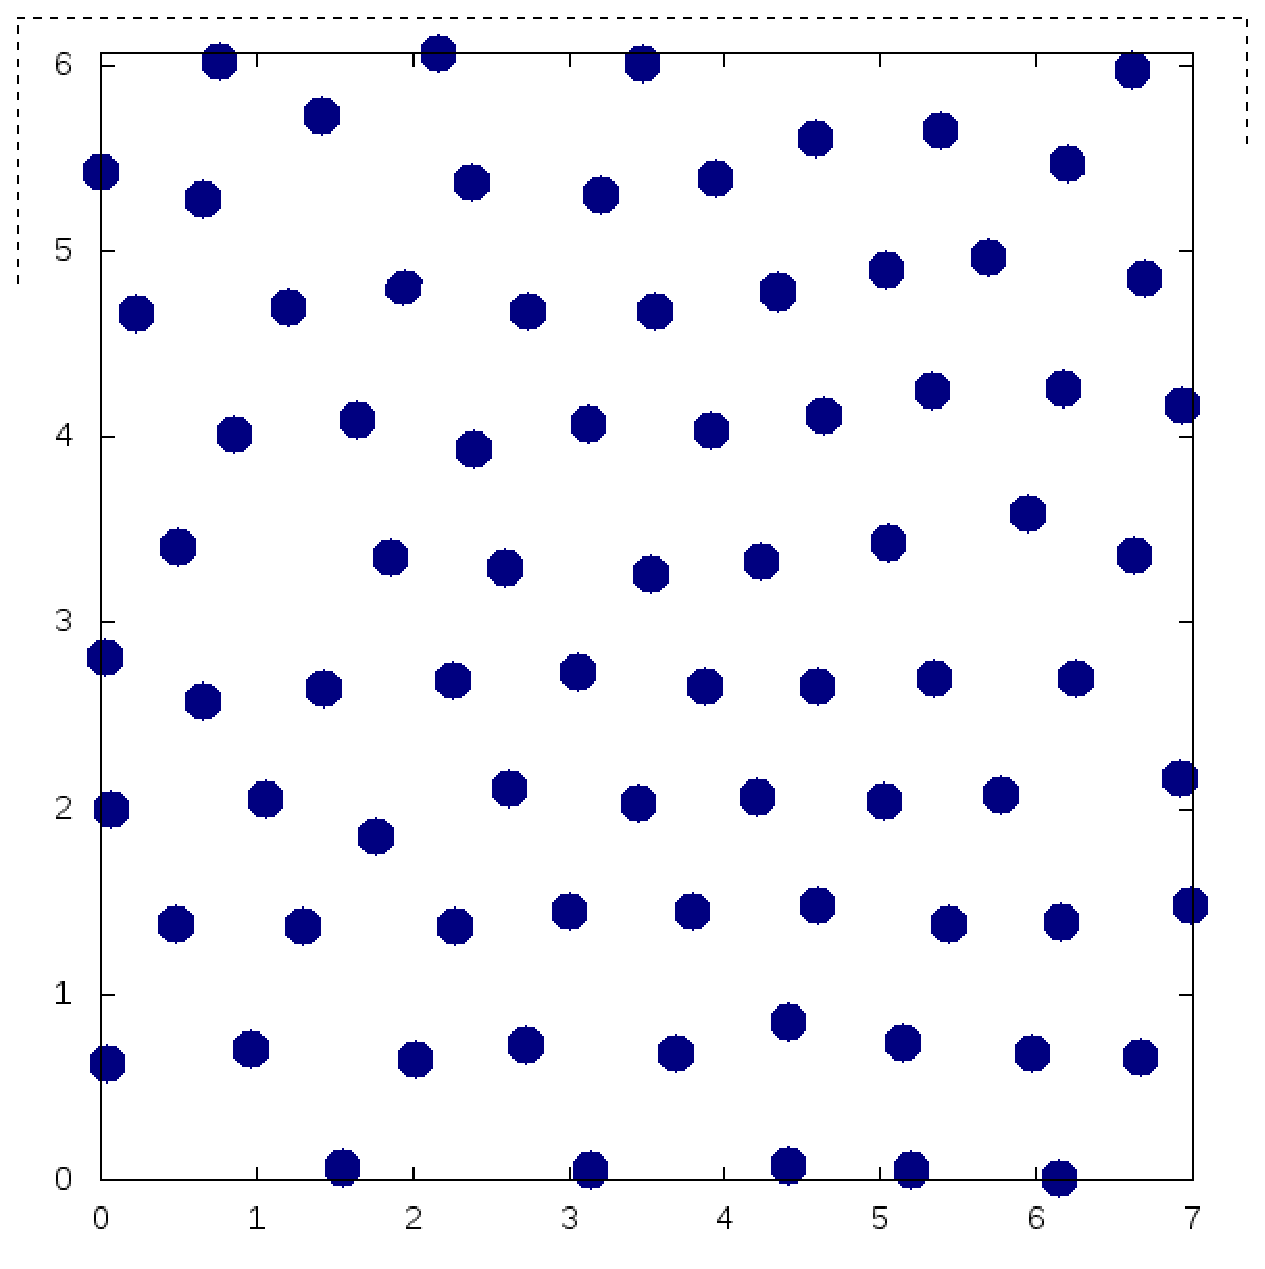
\includegraphics[width=1\linewidth]{pictures/system_dynamic_8_vac_kT005}}
\caption{Система с 6-ю вакансиями в ходе моделирования.}
\label{ris:image12}
\end{figure}
\begin{figure}[h]
\center{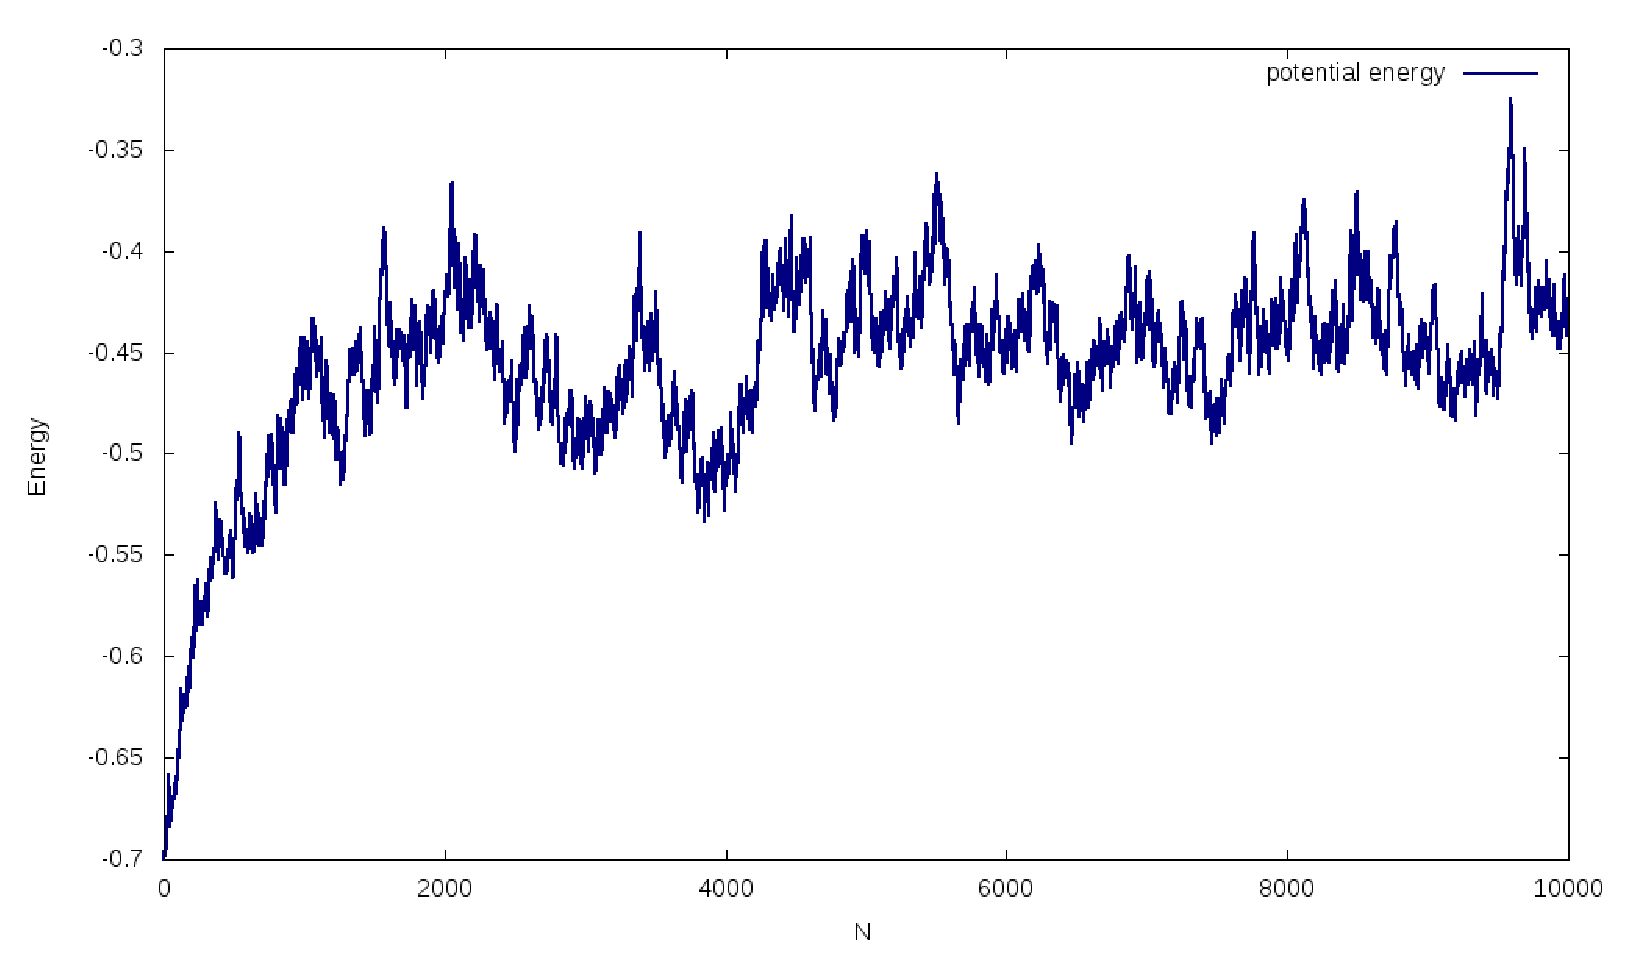
\includegraphics[width=1\linewidth]{pictures/energy_8_vac_kT005}}
\caption{График зависимости энергии системы с 6-ю вакансиями от шага моделирования.}
\label{ris:image13}
\end{figure}
\begin{figure}[h]
\center{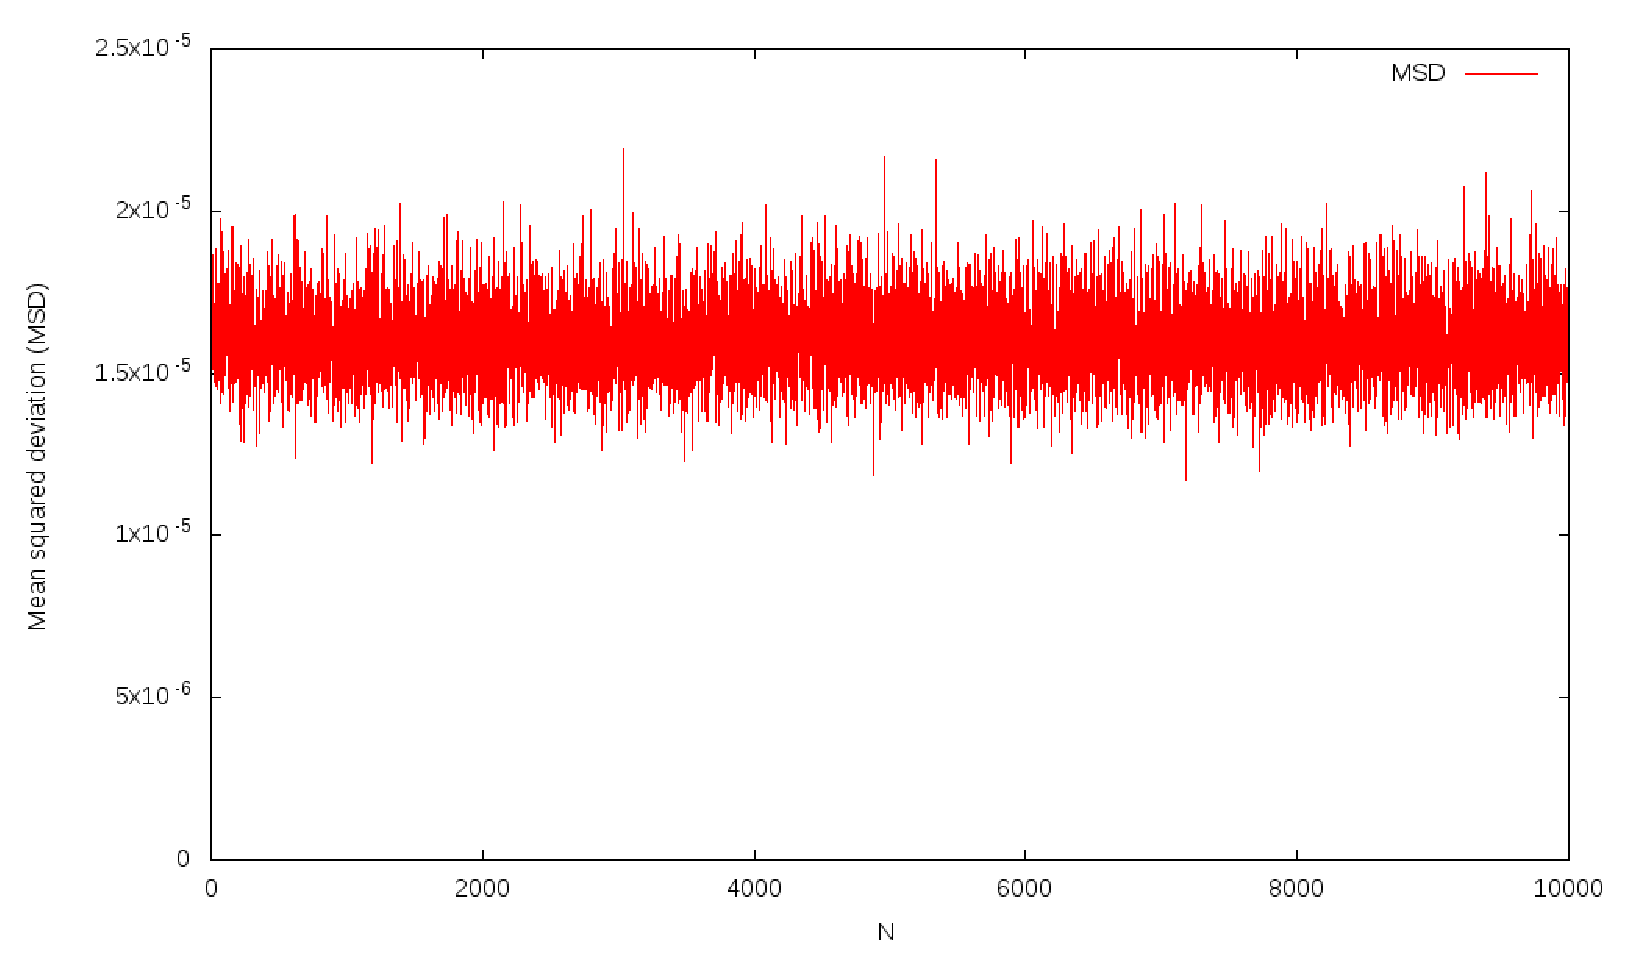
\includegraphics[width=1\linewidth]{pictures/MSD_8_vac_kT005}}
\caption{График зависимости среднеквадратического отклонения от шага моделирования.}
\label{ris:image14}
\end{figure}